% Use the article doc class, with an 11 pt basic font size
%\documentclass[11pt, a4paper, draft]{article}
\documentclass[11pt, a4paper]{article}
% Nice citations
\usepackage{natbib}
% Set margins
\usepackage[margin=2.5cm]{geometry}
% Multilingual support
\usepackage[english]{babel}
% Nice mathematics and Left-right harpoons for kinetic equations
\usepackage{amsmath,mathtools}
% Control over maketitle
\usepackage{titling,titlesec}
% Ability to use colour in text
\usepackage[usenames]{color}
\definecolor{grey}{rgb}{0.6, 0.6, 0.63}
\definecolor{black}{rgb}{0, 0, 0}
% For the \degree symbol
\usepackage{textcomp,gensymb}
% Allow includegraphics and wrapped figures
\usepackage{graphicx,wrapfig,subfigure}
\usepackage[outercaption]{sidecap}
\usepackage{csquotes}

%% Trick to define a language alias and permit language = {en} in the .bib file.
% From: http://tex.stackexchange.com/questions/199254/babel-define-language-synonym
\usepackage{letltxmacro}
\LetLtxMacro{\ORIGselectlanguage}{\selectlanguage}
\makeatletter
\DeclareRobustCommand{\selectlanguage}[1]{%
  \@ifundefined{alias@\string#1}
    {\ORIGselectlanguage{#1}}
    {\begingroup\edef\x{\endgroup
       \noexpand\ORIGselectlanguage{\@nameuse{alias@#1}}}\x}%
}
\newcommand{\definelanguagealias}[2]{%
  \@namedef{alias@#1}{#2}%
}
\makeatother
\definelanguagealias{en}{english}
\definelanguagealias{eng}{english}
%% End language alias trick

%% Any aliases here
\newcommand{\mb}[1]{\mathbf{#1}} % this won't work?
% Emphasis and bold.
\newcommand{\e}{\emph}
\newcommand{\code}[1]{\textsf{#1}}
\newcommand{\dvrg}{\nabla\vcdot\nabla}
%% END aliases

% Custom font defs
% fontsize is \fontsize{fontsize}{linespacesize}
\def\authorListFont{\fontsize{11}{11} }
\def\corrAuthorFont{\fontsize{10}{10} }
\def\affiliationListFont{\fontsize{11}{11}\itshape }
\def\titleFont{\fontsize{14}{11} \bfseries }
\def\textFont{\fontsize{11}{11} }
\def\sectionHdrFont{\fontsize{11}{11}\bfseries}
\def\bibFont{\fontsize{10}{10} }
\def\captionFont{\fontsize{10}{10} }

% Caption font size to be small.
\usepackage[font=small,labelfont=bf]{caption}

% Make a dot for the dot product, call it vcdot for 'vector calculus dot'. Bigger than \cdot, smaller than \bullet.
\makeatletter
\newcommand*\vcdot{\mathpalette\vcdot@{.35}}
\newcommand*\vcdot@[2]{\mathbin{\vcenter{\hbox{\scalebox{#2}{$\m@th#1\bullet$}}}}}
\makeatother

\def\firstAuthorLast{James}
\def\Address{\\
\affiliationListFont Department of Psychology,\\
 \affiliationListFont  The University of Sheffield, Sheffield, UK \\
}
\def\corrAuthor{Seb James}
\def\corrAddress{Department of Psychology, The University of Sheffield,
  Western Bank, Sheffield, S10 2TP, UK}
\def\Authors{\authorListFont Sebastian~S.~James, Stuart~P.~Wilson  \Address}
%  \corrAuthorFont $^{*}$ Correspondence: {seb.james@sheffield.ac.uk}}

% If no page numbering wanted:
%\pagenumbering{gobble}

% A trick to get the bibliography to show up with 1. 2. etc in place of [1], [2] etc.:
\makeatletter
\renewcommand\@biblabel[1]{#1.}
\makeatother

% reduce separation between bibliography items if not using natbib:
\let\OLDthebibliography\thebibliography
\renewcommand\thebibliography[1]{
  \OLDthebibliography{#1}
  \setlength{\parskip}{0pt}
  \setlength{\itemsep}{0pt plus 0.3ex}
}

% Define title, empty date and authors
\title {
Time to stop; agent-based modelling of chemoaffinity with competition
}
\date{} % No date please
\author{\Authors}

%% END OF PREAMBLE

\begin{document}
%\setlength{\droptitle}{-1.8cm} % move the title up a suitable amount
\maketitle

\emph{We show that a true chemoaffinity model based on gradient following (via receptor-ligand interactions) combined with receptor-ligand-mediated axonal repulsion, in which information is only transferred by nearest-neighbour interactions, can account for a broad range of experimental results.}



%\begin{itemize}
%    \item Sperry's chemospecificity model is an influential theory of how axons from neurons that originate in one tissue can find their way to specific locations in a target tissue during early brain development.
%    \item A key component of the theory is that growing axons find their way into position by chemotaxis, i.e., by evaluating local information in gradients of gene expression that span the target tissue
%    \item Computational models have shown that in addition to chemotaxis, local competitive interactions between growing axons can account for a wide range of results from experiments in which the factors known to influence the growth of axons have been surgically or genetically manipulated
%    \item However, while such models have \emph{assumed} the effects of chemotaxis, the key assumption of the chemospecificity model, that axons sample and evaluate positional information only \emph{locally}, is yet to be tested directly.
%    \item Consider, for example, an important model by Goodhill \& Simpson, which shows how [a certain set of assumptions about the form of the] competition between axons can account for patterns of innervation in the developing tectum that result from ablating/rotating sections of the retina.
%    \item The formulation of this model includes a term that at every time-step moves the simulated axons in the direction of a pre-specified target location. Thus the model implicitly assumes a global supervisor, capable of evaluating the current state of each axon, computing a direction vector to correct its trajectory, and communicating that information to each axon.
%    \item This model was constructed primarily to establish the effects of competition, and to this end is elegantly formulated.
%    \item Nevertheless, the key assumptions of the chemospecificity model, and specifically the proposal that axons find their way via evaluating only local information (chemotaxis), are yet to be investigated directly.
%    \item The aim of the current study is therefore to construct a model that represents the assumptions of the chemospecificity model explicitly.
%    \item One advantage of such a model is that it can be used to investigate the sensitivity and robustness of local interactions in establishing topographic maps to various sources of noise.
%    \item Indeed, our simulation results show that the local mechanisms of axonal information-processing that are assumed by the chemospecificity model provide a remarkably robust solution to the problem of topographic map development.
%\end{itemize}

\section{Introduction}

Sperry's chemoaffinity model is an influential theory of how axons from neurons that originate in one tissue can find their way to specific locations in a target tissue during early brain development \citep{sperry_chemoaffinity_1963}.
%
The central proposal of the theory is that growing axons find their location in a destination tissue by means of `labels of a cytochemical nature'.
The chemical affinity between labels in source and destination tissues allows axons to distinguish correct target locations from incorrect ones.
%
This key idea does not, on its own, explain how an axon can find the correct \emph{direction} in which it should move to reach its target.
An additional component of Sperry's theory \citep{gaze?} suggested that the axon could determine this direction by evaluating local information in gradients of gene expression spanning the target tissue, giving rise to chemotaxis of the axonal growth cones.
%
Sperry's theory was given robust support by the discovery of the ephrin ligands and their receptors \citep{cheng_complementary_1995,drescher_vitro_1995} which have been shown to form into graded expression fields in the retina \citep{braisted_graded_1997}, tectum \citep{braisted_graded_1997,feldheim_genetic_2000} as well as in other sensory systems, such as the somatosensory system \citep{vanderhaeghen_mapping_2000}.
%
The Ephrin ligands have a clear effect on axonal outgrowth, as shown in-vitro \citep{cheng_complementary_1995,drescher_vitro_1995,hansen_retinal_2004} and by in-vivo \citep{frisen_ephrin-a5_1998,rodger_transient_2000,mann_topographic_2002,hindges_ephb_2002} studies.

Computational models have shown that in addition to chemotaxis, local competitive interactions between growing axons can account for a wide range of results from experiments in which the factors known to influence the growth of axons have been surgically or genetically manipulated \citep{prestige_role_1975,simpson_simple_2011,suetterlin_target-independent_2014}.

However, while such models have \emph{assumed} the effects of chemotaxis, the key assumption of the chemoaffinity model, that axons sample and evaluate positional information only \emph{locally}, is yet to be tested directly.
%
Consider, for example, an important model by Goodhill \& Simpson, which shows how [a certain set of assumptions about the form of the] competition between axons can account for patterns of innervation in the developing tectum that result from ablating/rotating sections of the retina \citep{simpson_simple_2011}.
%
The formulation of this model includes a term that at every time-step moves the simulated axons in the direction of a pre-specified target location.
Thus the model implicitly assumes a global supervisor, capable of evaluating the current state of each axon, computing a direction vector to correct its trajectory, and communicating that information to each axon.
%
This model was constructed primarily to establish the effects of competition, and to this end is elegantly formulated.
%
Nevertheless, the key assumptions of the chemoaffinity model, and specifically the proposal that axons find their way via evaluating only local information (chemotaxis), are yet to be investigated directly.

The aim of the current study is therefore to construct a model that represents the assumptions of the chemoaffinity model explicitly.

One advantage of such a model is that it can be used to investigate the sensitivity and robustness of local interactions in establishing topographic maps to various sources of noise.

Indeed, our simulation results show that the local mechanisms of axonal information-processing that are assumed by the chemoaffinity model provide a remarkably robust solution to the problem of topographic map development.

\section{Results}
\subsection*{A model of chemotaxis and competition}

In an agent-based model of chemotaxis and competition, the position, $\mathbf{x}_t$, of each branch $b$ on a simulated tectum can be updated according to $\mathbf{x}_{t+1} = \mathbf{x}_{t} + \mathbf{M}$ with the movement vector $\mathbf{M}$ given by
\begin{equation} \label{e:mv2}
 \mathbf{M} = \mathbf{G} +  \mathbf{X} + \mathbf{B}.
\end{equation}
$\mathbf{G}$ is the movement due to the chemotaxis effect and $\mathbf{X}$ is the movement due to competitive interactions with other branches.
$\mathbf{B}$ is a movement applied close to the tissue boundary that ensures all branches remain within the tissue.

\citet{simpson_simple_2011} investigated a model of this form in which a `placeholder' provided a chemotaxis-like movement for $\mathbf{G}$ and a form for $\mathbf{X}$ was studied.
Their model, which successfully accounts for a wide range of experimental manipulations, found an $\mathbf{X}$ comprised of two components; a simple distance-based competition between \emph{all} branches ($\mathbf{C}$), along with an axon-axon interaction based on the relative levels of the receptor EphA expressed by each interacting axon ($\mathbf{I}$).
We asked i) if the placeholder mechanism for $\mathbf{G}$, in which a `global supervisor' informs each branch of the vector along which it should travel to approach its target, could be replaced by a true chemotaxis mechanism based on graded signalling molecule expression and ii) if the competition mechanism found by Simpson and Goodhill was the simplest possible mechanism that could explain all of the surgical and genetic manipulations accounted for by their model.

\subsection*{A gradient based model of chemotaxis}

We assumed a purely linear receptor binding model, and set the chemotactic movement vector of the branch $b$ at location $\mathbf{x}$ on the tectum to be

\begin{equation}\label{e:G}
\mathbf{G} = m_{\!_G}\,\sum_i^N F_i\,r_{i,b} \nabla L_i(\mathbf{x})
\end{equation}
%
where $r_{i,b}$ is the receptor expression on branch $b$ for ligand-receptor pair $i$, $L_i$ is the expression of ligand $i$ on the tectum and $F_i$ denotes the direction of the interaction induced when a molecule of ligand $i$ binds to a receptor $i$ molecule.
$F_i$ takes the value $-1$ for a repulsive interaction or $1$ for an attractive interaction.
%
We assumed that all receptor-ligand signalled interactions are repulsive ($F_i=-1, \forall i$), as for EphA-ephrinA coupling \citep{drescher_vitro_1995,nakamoto_topographically_1996}.
%
$m_{\!_G}$ is a scalar parameter which controls how much movement is generated for a given level of receptor-ligand gradient signalling.

%%%%% Describing the simulation
We simulated the retina and tectum as unit square regions and defined retinal receptor expression and tectal ligand expression across these squares (Fig.\,\ref{f:ex}B-D).
The simulated retina possessed $n$=400 (20$\times$20) retinal ganglion cells; the tectum was similarly arranged as 20$\times$20 discrete, square elements, with defined levels of expression for each ligand.
One spatial unit corresponds to 2~mm on the retina or tectum for mouse \citep{reber_relative_2004}.

Each retinal ganglion cell (RGC) projects $M=4$ growth cones (referred to as \emph{branches}) which carry a set of $N$ receptors, $r_i$ indexed by $i$ and expressed at levels determined by the cell soma's location on the retinal grid.
($N$ ligands, $l_i$, are also expressed by RGCs, but these are not used for chemotaxis.)
The expression of each receptor varies only with respect to one spatial dimension.
%
We defined 4 receptor expression gradients arranged in orthogonal pairs with the gradient of $r_0$ being orthogonal to that of $r_1$. $r_2$, whose gradient is opposite to $r_0$, was orthogonal to $r_3$ (Fig.\,\ref{f:ex}B).
%
Because there is convincing evidence that EphA and EphB receptors are expressed in exponentially increasing patterns \citep{reber_relative_2004,feldheim_genetic_2000,brown_topographic_2000,koulakov_stochastic_2004}, we use an exponential form for retinal receptor expressions, in common with other modelling studies~\citep{reber_relative_2004,koulakov_stochastic_2004,simpson_simple_2011}.
We adopt the same precise form for the retinal receptor expression as \citet{simpson_simple_2011}, $f(x,y) = 1.05 + 0.26 \exp(2.3 u)$, where $u$ gives the direction with which the expression increases and is substituted by $(1-x)$ for $r_0$, $(1-y)$ for $r_1$, $x$ for $r_2$ and by $y$ for $r_3$ (Fig.\,\ref{f:ex}B).

Cells on the tectum express ligands, $L_i$, for the retinal receptors, also in orthogonal pairs of gradients.
Although several studies model tectal ligand expression with exponential functions \citep{koulakov_stochastic_2004}, the experimental evidence for the form of tectal ligand expression is more ambiguous than that for retinal receptor expression (Fig.\,\ref{f:expressions} summarises results from the literature).
We kept in mind the possibility that tectal ligand expression may be modelled by another function, but initially, we set it to the same exponential used for retinal expression and used the substitutions $y$, $x$, $(1-y)$ or $(1-x)$ in place of $u$ to obtain the ligand expression functions for $L_0$, $L_1$, $L_2$ and $L_3$ (Fig.\,\ref{f:ex}D).

While we do not explicitly name $r_0$, $r_1$, etc.~as \emph{EphA}, \emph{EphB}, the suggestion is that $r$ includes EphA, EphB, Ryk \citep{schmitt_wntryk_2006} and Neogenin \citep{rajagopalan_neogenin_2004} receptors and that $L$ includes the ephrin-A, ephrin-B, Wnt3 \citep{schmitt_wntryk_2006} and RGM \citep{monnier_rgm_2002} ligands, each of which has been shown to play a r\^ole in retinotectal map formation.

\subsection*{A signalling model for competition}

 We modelled competition as distance-based competitive movement vector, $\mathbf{X}$, which is `switched on' via receptor-ligand signalling:
%
\begin{equation}
\mathbf{X} = \frac{m_{\!_X}}{|B_{b}|} \sum_k^{nM} \hat{\mathbf{x}}_{kb}\,W\,Q(d_{kb}, \mathbf{r}_{b}, \mathbf{l}_{k}).
\end{equation}
%
$W$ is the distance based weighting ($W = 1-\frac{d_{kb}}{2r_{\!_X}}~\mathrm{if}~  d_{kb}\leq 2r_{\!_X}$) and $B_{b}$ is the set of branches that are within interaction distance of $b$. $m_{\!_X}$ is a scalar parameter, $nM$ is the total number of branches and $\hat{\mathbf{x}}_{kb}$ is the unit vector from $k$ to $b$.
%
$Q$ is a signalling threshold function which depends on the distance $d_{kb}$ between two branches $b$ and $k$, the receptor expression on $b$ ($\mathbf{r}_b$) and the ligand expression on $k$ ($\mathbf{l}_k$):
%
\begin{equation}
Q(d_{kb}, \mathbf{r}_{b}, \mathbf{l}_{k}) = \begin{cases}
                 0 & \mathrm{if}~-F_i\,r_{i,b}\,l_{i,k} <
                 s,\,\forall{i}~\mathrm{or}~d_{kb} > 2r_{\!_X} \\
                 1 & \mathrm{otherwise.}
     \end{cases}
\end{equation}
%
$r_{\!_X}$ is the receptor-ligand interaction radius, $l_{i,k}$ (the expression of ligand $i$ on branch $k$) is the $i^{\mathrm{th}}$ element of $\mathbf{l}_k$ and $r_{i,b}$ is the $i^{\mathrm{th}}$ element of $\mathbf{r}_b$.
$F_i$, defined in Eq.\,\ref{e:G}, is -1 if the $r_{i}\,l_{i}$ interaction signals repulsion and +1 if it signals attraction.
$s$ is a positive signal threshold for interaction.
With the constraint $s>0$ comes the assumption that attractive interactions will have no effect on the competitive movement vector---a receptor-ligand pair that signals attraction cannot cause $Q$ to take the value 1.
$Q$ is set to 1 only if at least one repulsive signal exceeds $s$ and the distance from branch $b$ to branch $k$ is smaller than $2 r_{\!_X}$.

\subsection*{Simulation}

The model has four free parameters; $m_{\!_G}$, $m_{\!_X}$, $r_{\!_X}$ and $s$. We fixed $m_{\!_G}$ to the value $0.0012$ and used the optimization to find the competition parameters that would balance this level of chemotaxis.
To find the best combination of the remaining three parameters, we reasoned that evolution would optimize the arrangement of the wildtype pattern.
We performed a simulated annealing optimization to minimize an objective function for the wildtype pattern (Fig.\,\ref{f:GJ}E) at simulation time 1000.

We used a combination of pattern metrics to define the objective function. $\epsilon$ is the mean distance error of the axon centroids, given by:
%
\begin{equation}\label{e:eps}
\epsilon = \sqrt{\frac{\sum_k^n (\mathbf{x}_{k} - \mathbf{x}'_{k})^2}{n}},
\end{equation}
%
where $\mathbf{x}_{k}$ is the location of the centroid of the branches of axon $k$ and $\mathbf{x}'_{k}$ the target tectal location for axon $k$.
$n$ is the number of RGC axons in the system.
%
$\epsilon$ tends to 0 as the pattern approaches the target layout.
However, two patterns may have the same non-zero value for $\epsilon$, despite one being qualitatively more disordered than the other.
For this reason, we also use the number of crossings in the fish net plot of the axon centroids (see Fig.\,\ref{f:GJ}D) as a second metric, called $\eta$, which tends towards an expected target number of crossings, $\eta_t$ as the pattern approaches the target layout. The annealing objective function, $\xi$, combined these metrics with $\xi = \epsilon^2 (1+\frac{\eta}{100})$.
The parameters returned by the simulated annealing were
$m_{\!_X} = 0.2078$, $r_{\!_X} = 0.0759$ and $s = 4.815$.

Fig.\,\ref{f:GJ} shows the simulation results with these parameters after 1500 time steps.
Fig.\,\ref{f:GJ}A indicates the colour code used for retinal cell position; dorsal retinal cells are indicated by green, nasal cells by red. Lightness gives position along the relevant axis so that cells at the dorsal-nasal corner are yellow and those at the ventral-temporal corner are black.
Fig.\,\ref{f:GJ}E shows the expected layout of retinal ganglion cell axons on the tectum.
The axons retain the colour of their originating cell on the retina.
Nasal cell axons should be arranged caudally; dorsal axons laterally; axons should be evenly spaced and the pattern should span the entire tectum.
Fig.\,\ref{f:GJ}, panels B--D show `fish net' plots of the average location of the 4 branches of each axon (the axon's centroid) at three timepoints.
Fig.\,\ref{f:GJ}B indicates the randomised placement of axon branches at the rostral end of the tectum as specified by the initial conditions (Eq.\,\ref{e:ic}).
In these plots, lines are drawn between axons that are expected to arrange themselves adjacently to one another by the end of the simulation.
The number of line crossings in this plot gives an indication of the disorder in the arrangement.
Fig.\,\ref{f:GJ}G shows the positions of the individual branches (i.e.~growth cones) at $t=1500$ that contribute to the plot in Fig.\,\ref{f:GJ}D.
By this time, the topological order matches that shown in Fig.\,\ref{f:GJ}E.
Opposing gradients have sorted the axons along the two axes to form a grid of cells.
The arrangement spans the full tectum due to competition between the growth cones (\textbf{ref supp. figure of chemo-only model}).
Fig.\,\ref{f:GJ}F shows the two pattern metrics; $\epsilon$ (distance error) and $\eta$ (number of crossings).
For the wildtype pattern, $\eta_t=0$, as in Fig.\,\ref{f:GJ}E.
Fig.\,\ref{f:GJ}H shows selected axons (one from the centre and one from each corner of the retina) and their position history.

\subsection*{Surgical manipulations}

After finding an optimum set of parameters for the wildtype arrangement, we tested our model with a number of simulations of surgical manipulations (for reviews, see \citet{udin_formation_1988} and \citet{goodhill_retinotectal_1999}).
Figs.~\ref{f:GJsurg}A and \ref{f:GJsurg}B show the results of tectal graft rotation manipulations in which a square patch of tectal tissue is cut out and rotated $90\degree$ or $180\degree$ \citep{chung_observations_1978}.
%
To simulate the surgery, we rotated an $8\times8$ square of the tectum shown in Fig\,\ref{f:ex}D, carrying the ligand expressions with the rotation (resulting in Fig.\,\ref{f:trot90}, left column).
After the manipulation, we re-computed the tectal ligand expression gradients. Fig.\,\ref{f:trot90} demonstrates that the most significant change in the gradient is around the border of the graft, due to discontinuities in the ligand expression.
The manipulated gradients, interacting with unchanged axon branches, lead to a qualitative rotation of axons that were destined for the graft area, indicated by a 90$\degree$ or 180$\degree$ `twist' of the axon centroid colours.
Long connecting lines in the fish net show that a number of axons from near the edges of the tectum have been drawn into the graft region.
The pattern metric, $\epsilon$, is shown in the right hand graphs of Fig.\,\ref{f:GJsurg}A \& B.
We plot $\epsilon$ (the distance error) for the entire map (blue) along with the error for the graft region (gold) and the surround region (red).
The overall distance error for the rotation manipulations (0.182 or 0.2752)  is greater than for the wildtype system (0.04).
The pattern within the graft exhibits greater average distance error than for the surrounding tissue.
The system does not achieve a perfect reproduction of the target layout suggested by the experimental result (which is shown in the inset) but it is in qualitative agreement.
%
Fig.\,\ref{f:GJsurg}C shows the result of a similar manipulation in which two grafts are cut out of the tectum and swapped. \textbf{Fixme: which of the two grafts does the RH graph refer to?}

Fig.\,\ref{f:GJsurg}D shows the result of a retinal ablation, in which the temporal half of the retina is surgically removed and the remaining RGC axons are allowed to develop on the unmanipulated tectum.
According to a pure chemoaffinity theory, the surviving retinal axons should retain their chemical labels and they would be expected to find their usual locations on the tectum, resulting in a tectum which is only half populated with axons.
The experimental observation is that the axons arrange themselves across the whole tectum, retaining their topographic order (inset) \citep{attardi_preferential_1963,schmidt_expansion_1978}.
The fish-net plot of the simulation indicates that the competition in the system successfully `stretches out' the surviving axons to achieve a close representation of the experimentally observed result.
In this figure, the right-hand graph shows the simulated position of each axon centroid on the rostro-caudal tectal axis plotted against its position on the nasal-temporal retinal axis in red triangles, with the experimental positions plotted in blue squares.
%
Fig.\,\ref{f:GJsurg}E shows the result of a tectal ablation. Here the retina is left un-modified, but the caudal half of the tectum is surgically removed. Experimental observation \citep{yoon_reorganization_1971,sharma_reformation_1972} shows that RGC axons `crush up' on the remaining rostral section, retaining topographic order and creating a complete map on the available tectal tissue. Our model clearly replicates this result, indicated by both fish-net and tectal/retinal axes graphs, because the chemotaxis component of the model is based on balanced, relative interactions between opposing gradients, rather than absolute labels or expression measurements.
%
A related ablation experiment is the so-called `mismatch', in which the temporal half of the retina is ablated along with the caudal part of the tectum to which it normally maps, again challenging the pure chemoaffinity model \citep{horder_retention_1971}. Our model replicates this manipulation (Fig.\,\ref{f:GJsurg}F) for the same reason as in the simple tectal ablation of Fig.\,\ref{f:GJsurg}E; opposing gradients remain on the surviving tectum allowing RGC axons to find their relative ordering.
%
The final surgical manipulation which we investigated was the `compound eye' experiment, in which two nasal retina halves are fused together \citep{gaze_retino-tectal_1963,fawcett_retinotectal_1982}. Within the compound retina there exist matched pairs of retinal ganglion cells, one from each nasal half, whose receptor and ligand expressions cannot be distinguished. These form overlaid maps, each of which spans the entire tectum (Fig.\,\ref{f:GJsurg}G).

\subsection*{Genetic manipulations}

In the early 2000s, a series of genetic experiments added to the set of manipulations that a model of the retinotectal system would need to
explain.
First, \citet{brown_topographic_2000} showed that a selective RGC knock-in of EphA3 receptors led to an interesting modulation of the maps found in the tectum.
For the strongest knock-in (a homozygote manipulation) two maps were formed, with knock-in cells finding termination zones more rostral than their wildtype retinal neighbours.
By enhancing the quantity of EphA receptors expressed by half of all retino-tectal axons, they demonstrated the importance of retinal receptor expression for the arrangement of the tectal map.
In the weaker, heterozygote manipulation, the maps were still separated, but the separation `collapsed' towards the rostral end of the tectum (see \citet{brown_topographic_2000}, Fig\,5).
This led to a second study showing that with an additional knock-down of EphA4 receptors in \emph{all} RGCs, the retinal origin of the collapse point was shifted temporally and all heterozygote EphA3 knock-in cells were pushed even further rostrally (\citet{reber_relative_2004}, their Fig.\,3e).
Does our model reproduce the results of Brown et al and Reber et al?

An assumption made in these papers is that all EphA receptor subtypes contribute to a summed EphA expression level, $\sum\mathrm{EphA}$, which increases from a low level at the nasal side of the retina, to a high level at the temporal side.
The precise contribution of each subtype to the overall level is assumed not to be important.
In our model, receptor $r_0$ increases in the retina in a nasal to temporal direction (Fig\,\ref{f:ex}B) and so we will manipulate $r_0$ to recreate the Brown et al.~and Reber et al.~experiments.
In half of the RGCs, we knock-in EphA3 by adding to the value of $r_0$ in these cells either 0.6 (heterzygote EphA3 ki/+) or 3.0 (homozygote EphA3 ki/ki).
To add the additional knock-down of EphA4 in \citet{reber_relative_2004}, we subtract 0.35 from $r_0$ in \emph{all} RGCs.
Fig.\,\ref{f:GJeph}A-C shows, for the single EphA3 knock-in (EphA3 ki/+), branch positions, axon centroids and final rostral-caudal position on the tectum plotted versus the originating nasal-temporal retinal coordinate.
In A, branches are coloured in the red/green duochrome scheme according to their origin location on the retina.
In B \& C, axon centroids of RGCs which were treated with the knock-in manipulation are coloured red, wildtype cells are blue.
The map of treated cells on the tectum is shifted slightly rostrally, but the shift becomes statistically insignificant at about 0.75 along the nasal-temporal axis.
While the map collapse is less abrupt than in the experimental result of \citet{brown_topographic_2000}, it is comparable with the result from \citet{simpson_simple_2011}.
Fig.\,\ref{f:GJeph}D-F shows the same trio of graphs for the homozygote double knock-in, EphA3 ki/ki. Here, the treated axons are pushed further towards the rostral end of the tectum and the untreated axons are pushed caudally.
The maps are completely separated; as in the experiment, there is no `collapse point'.

The rostral movement of treated axons occurs due to their increased expression of EphA ($r_0$), which increases the interaction with the tectal rostral-caudal ligand gradient.
The opposing receptor expression ($r_2$) is unchanged by the manipulation and so those axons with increased $r_0$ expression are pulled to a more rostral position than they would otherwise take.
The caudal movement of wildtype axons, whose receptor expression in Figs.\,\ref{f:GJeph}A-F is unchanged, occurs due to competition with the caudally-drawn treated axons.

Figs.\,\ref{f:GJeph}G-I show the results for the Reber et al.~manipulation, in which the EphA expression is selectively knocked in in 50\% of cells and knocked down in all cells.
The collapse point has moved from about 0.75 in Fig.\,\ref{f:GJeph}C to about 0.85 (\textbf{check}), in agreement with the
experimental result.
However, the significant rostral movement of the treated axons seen in \citet{reber_relative_2004}, where not a single treated axon was found more than 30\% along the rostral-caudal axis, was absent from our result.

\section{Discussion}

\subsection*{On chemotaxis}

Gradient based model discussed, but not simulated by \citet{hope_arrow_1976}.

\citet{nakamoto_topographically_1996} is Gradient based model.

The minimum number of gradients required to provide a coordinate system on the surface of the tectum within which axons could find a target location is $N=2$, arranged in orthogonal directions.
However if there are only two gradients, imagining that one guides axons laterally and the other guides axons in the caudal direction, then it is necessary for there to be an additional `stopping mechanism' to prevent all of the axons eventually being guided to the most lateral/caudal position.
To avoid the need for a different stopping mechanism, we chose to model \emph{opposing pairs of orthogonal gradients} with $N=4$.
With opposing gradients, an axon which interacts most strongly with a gradient in the caudal direction would be drawn to the caudal side of the tectum, whereas an axon whose strongest interaction was to climb a gradient in the rostral direction would be drawn to the rostral side.
There is evidence that multiple gene expression gradients are found in the brain, with examples of opposing pairs including XX and YY.
Adopting a pair of opposing gradients is mathematically reminiscent of the models of \citet{gierer_model_1983} which proposed... and \citet{fraser_differential_1980}.

\subsection*{Chemotaxis in isolation}

\subsection*{On competition}

Because many of the ligands expressed on the tectum are also expressed by retinal ganglion cells, there exists the possibility for inter-RGC signalling via receptor-ligand binding (forward interactions).
We chose to model this kind of interaction between RGCs, noting that if a forward interaction on the tectum leads to growth cones moving away from a region of high ligand expression (ephrin-A/EphA interactions act in this way), then the equivalent axon-axon interaction would also be expected to be repulsive. An interaction between one branch dense with receptors and another with a large number of ligands would have a high chance of repelling; an interaction between branches each with low levels of receptor/ligand expression would have a low chance of repelling.


Note that $\mathbf{X}$ would be equivalent to Simpson \& Goodhill's $\mathbf{I}_b$, which is a threshold-activated signal based on the ratio of $r_{i,b}/r_{i,k}$, if there was a single $l_i$ expressed in the retina and its form was $1/r_i$.
However, because we intended for $\mathbf{X}$ to be the only mechanism for competition, we found that the minimum number of ligands that were required to be expressed on the retina was 2, expressed in opposing directions (Fig.\,\ref{f:ex}C). If only a single receptor-ligand pair participated in competition, then many axons experienced no competitive interaction and such a system was unable to reproduce experimental observations.

\subsection*{Single axon behaviour}

\subsection*{Attractive receptor-ligand interactions}

\subsection*{The value of $s$}

% Bibliography here
\selectlanguage{English}
\bibliographystyle{apalike}
\bibliography{RetinoTectal}

\appendix

\section*{Method details}

\subsection*{Border effect} % border effect description
The border effect is also based on gradient following by assuming that there is some other molecular signal which acts on all branches near the boundary of the tectal tissue. For a branch with position $(x,y)$, $\mathbf{B}$ is given by:
%
\begin{equation}\label{e:B}
B_x = \begin{cases}
        \frac{1}{2} (r-x)     & x<r \\
        \frac{1}{2} (1-r-x)    & x>1-r
\end{cases}
B_y = \begin{cases}
        \frac{1}{2} (r-y)      & y<r \\
        \frac{1}{2} (1-r-y)    & y>1-r
\end{cases}
\end{equation}
%
Thus $\mathbf{B}$ is equivalent to the action of a repulsive signalling molecule expressed around the border of the tectum, whose expression increases quadratically outside the tectum and affects any branch touching (or outside) the boundary.
% end border effect description

\subsection*{Initial conditions}
Branches were initially randomly distributed in a stripe at the rostral side of the tectum at the start of each simulation.
Each RGC axon $k$ was assigned a random initial position coordinate:
\begin{equation}\label{e:ic}
\mathbf{x}_{k,t=0} = (U(0,1), U(-0.2,0))
\end{equation}
where U(p,q) is a number selected from a random uniform distribution in the range $[p,q)$. Each of the 4 branches per RGC axon was given its parent axon's initial position, plus a randomly generated offset with coordinates derived from a normal distribution of mean 0 and standard deviation 0.1.
% end initial conditions


%
% FIGURES
%

% FIGURE 1
\begin{figure}

\includegraphics[width=\linewidth]{./images/expressions_fig.png}
\caption{Simulated retinal and tectal signalling molecule expression.
\textbf{A} A schematic of retino-tectal mapping.
%
\textbf{B} Retinal receptor expression, $r_i$. Four receptors are expressed and displayed here in two dual-colour maps. $r_0$ and $r_1$ are red and blue; $r_2$ and $r_3$ are cyan and magenta. $r_0$ increases as an exponential function of $-x$; $r_1$ increases with an exponential function of $-y$. $r_2$ and $r_3$ have the opposite sense. Retinal receptor expression is modelled with exponential functions because there is ample evidence to support this form. $N$: nasal, $T$: temporal, $D$: dorsal, $V$: ventral.
%
\textbf{C} Retinal ligand expression, $l_i$, is expressed in complimentary gradients \citep{hornberger_modulation_1999}.
%
\textbf{D} Tectal ligand expression $L_i$. Tectal ligand expression is shown in an exponential form, although there is less evidence to determine whether tectal expression is exponential, linear or logarithmic.
$L$: lateral, $M$: medial, $C$: caudal, $R$: rostral.
}
\label{f:ex}
\end{figure}

% FIGURE 2
\begin{figure}
\includegraphics[width=\linewidth]{./images/j4_ee_GJ_best_1_wt_fig2_exit_true_steps_1500.png}
\caption{Receptor-ligand model of chemotaxis and competition.
\textbf{A} The origin position on the tectum gives axons a colour according to a dual-colour map. Axons in panels B-H that are red are those which originated in the most naso-ventral corner of the square simulated retina.
\textbf{B}-\textbf{D} Axon centroid positions on the simulated tectum (dashed line) at time 0, 40 and 1500 units. Lines show adjacency relationships between the axons' origin positions on the retina.
\textbf{E} Layout of axon centroids on the tectum observed in experimental results.
\textbf{F} The sum-of-squared difference error, $\epsilon$, and the number-of-crossings error metric, $\eta$ of the tectal axon arrangement plotted with respect to simulation time.
\textbf{G} The arrangement of axon branches at t=1500.
\textbf{H} Selected axon locations at t=1500, with path histories in grey.
\emph{Abbreviations: D dorsal, V ventral, T temporal, N nasal, C caudal, R rostral, M medial, L lateral.}}
\label{f:GJ}
\end{figure}

% FIGURE 3 ./scripts/fig_GJ_surgical.sh
\begin{figure}

\includegraphics[width=\linewidth]{./images/fig_GJ_surgical.png}
\caption{$\mathbf{GJ}$ model, surgical manipulations}
\label{f:GJsurg}
\end{figure}

% FIGURE 4
\begin{figure}
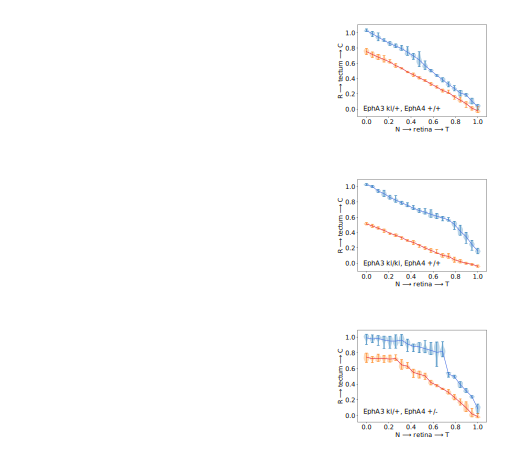
\includegraphics[width=\linewidth]{./images/EphA_manipulations.png}
\caption{$\mathbf{GJ}$ model, Brown et al./Reber et al.~manipulations.}
\label{f:GJeph}
\end{figure}

% ANY SUPPLEMENTARY FIGURES GO AFTER THIS
\renewcommand{\thefigure}{S\arabic{figure}}
\setcounter{figure}{0}

\begin{figure}
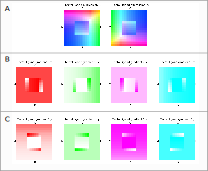
\includegraphics[width=\linewidth]{./images/Tissuevisb.png}
\caption{Ligand expression and gradients on the tectum for the
graft-rotate 90 degrees simulated surgical manipulation}
\label{f:trot90}
\end{figure}

\end{document}
